


\chapter{Computer Vision}
\label{sec:vision_pipeline}

To enable closed-loop alignment of the gantry end-effector to moving objects on the conveyor, a lightweight computer vision (CV) pipeline was developed in simulation using OpenCV. The primary goal of the pipeline is to estimate the target object's 2D pose in the image: \textit{(i)} center location in pixel coordinates $(u,v)$ and \textit{(ii)} in-plane orientation $\theta$ (yaw) using a minimum-area rectangle fit. This estimate is then used by the downstream alignment/visual servoing module.

A lightweight computer vision pipeline has been developed in simulation using OpenCV, so that closed-loop alignment of the gantry end-effector to moving objects can be performed. The goal is to estimate the target's 2D pose in the image; first, the center location in pixel coordinates $(u,v)$, then the orientation $\theta$ (yaw) through a minimum-area rectangle fit. This estimate is then what is used for downstream alignment using visual servoing.

Figure~\ref{fig:vision_pipeline_flow} summarizes the full image-processing pipeline. The camera mounted on the wrist obtains the input frame, which is then processed to segment the target object (such as brown cardboard or black microwaves), remove noise, and then estimate the pose.

\begin{figure}[H]
    \centering
    % Replace with your exported Lucid image filename
    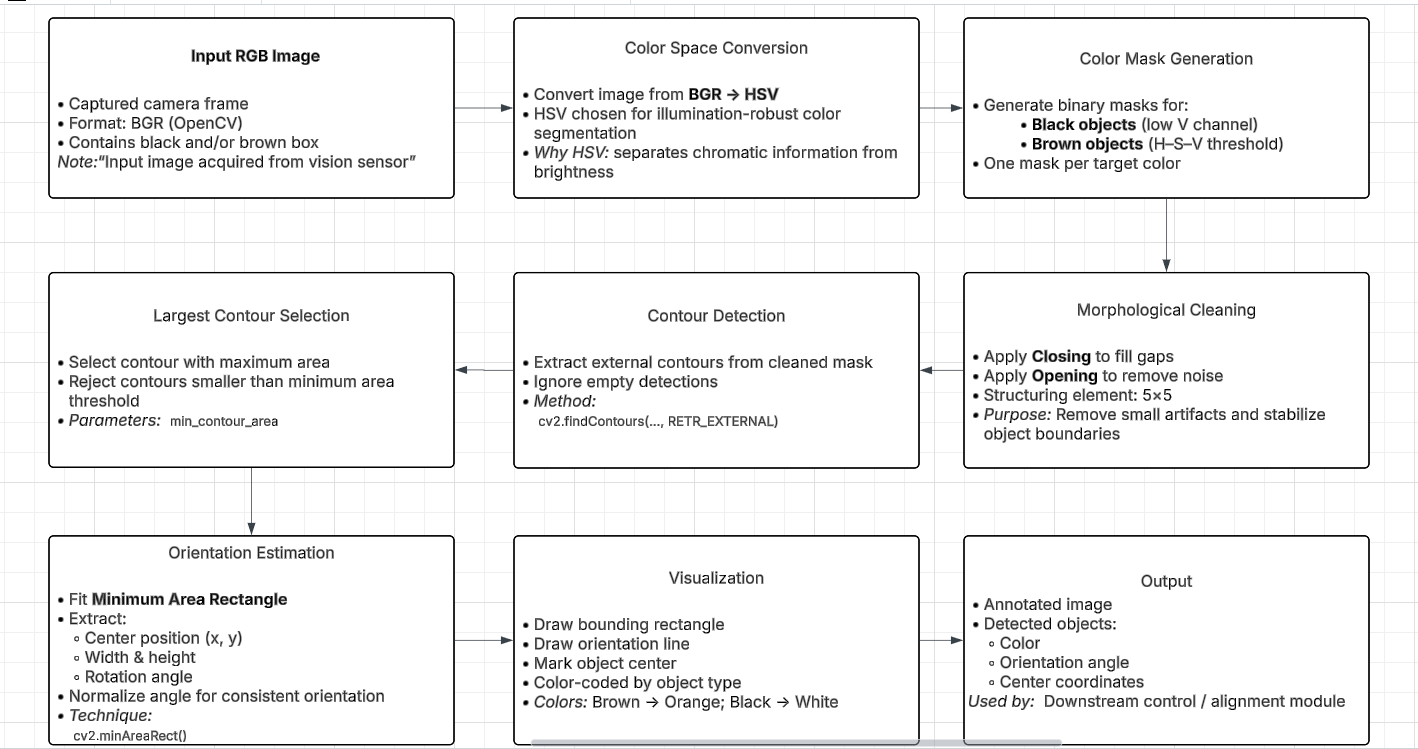
\includegraphics[width=\linewidth]{figures/vision_pipeline.png}
    \caption{Computer vision pipeline for segmentation and pose estimation using HSV thresholding, morphological filtering, contour extraction, and minimum-area rectangle fitting.}
    \label{fig:vision_pipeline_flow}
\end{figure}

The captured image is converted to HSV color space. This is done so that if the camera experiences changes in lighting, the processing can stay robust. Binary masks are then generated using thresholding, where the black object mask thresholded primarily on the Value channel for dark region isolation, while the brown object mask used a constrained HSV range tuned for the brown color of cardboard boxes. This way, the pipeline could detect objects of specific colors without resorting to data-hungry deep learning techniques based on inference.

However, small artifacts remain, so the binary mask is cleaned with standard morphological operations. This includes both closing to fill small gaps and opening to remove isolated noise. Then, a $5\times 5$ structuring element is used; depending on the noise, multiple iterations are run.

This leads to a position where external contours can be obtained. This is done using \texttt{cv2.findContours(..., RETR\_EXTERNAL)}. The pipeline extracts the contour with the greatest area; any other contours are rejected as false detections. This selected contour is fit using \texttt{cv2.minAreaRect}, obtaining at last:
\begin{itemize}
    \item Center in pixels: $(u, v)$
    \item Rectangle dimensions: $(w, h)$
    \item Raw angle: $\theta_{\text{raw}}$
\end{itemize}
However, OpenCV's angle convention depends on the longer edge (width or height). Hence, the raw angle is normalized, so that the pipeline supplies a consistent orientation $\theta \in [0,180)$.

Typical PID control needs world coordinates, but the coordinates just obtained are in the camera frame. Therefore, an IBVS formulation is selected, because it directly operates on pixel coordinates by minimizing the error between current image features and the desired ones. For a feature vector $s=[x\;\;y\;\;\theta]^T$ (or alternatively $[u\;\;v\;\;\theta]^T$), the control objective is to reduce:
\[
e = s - s^{*}
\]
where $s$ is measured from the current camera frame and $s^{*}$ is the desired feature. In this case, this is the target centered in the image with desired yaw.

First, $(u,v)$ can be converted to normalized image coordinates:
\[
x = \frac{u - c_x}{f_x}, \quad y = \frac{v - c_y}{f_y}
\]
and then the interaction matrix maps camera velocities to feature motion:
\[
\dot{s} = L_s \, v
\]
Finally, a standard IBVS control law is used:
\[
v = -\lambda \, L_s^{+} \, e
\]
where $\lambda>0$ is a gain and $L_s^{+}$ is the pseudo-inverse of the interaction matrix. With only camera measurements and no availability of actual object pose in world coordinates, closed-loop alignment can be done.

The image processing pipeline performed well on simulation, so this was dispatched on a real Dawlance microwave and its repective box. While the orientation was correctly obtained (to the nearest half degree), the position encountered minor but not negligible errors because of the flaps of the box and the sides of the microwave. Hence, while this algorithm is effective, it needs further tuning to handle these real cases.

\begin{figure}[H]
    \centering
    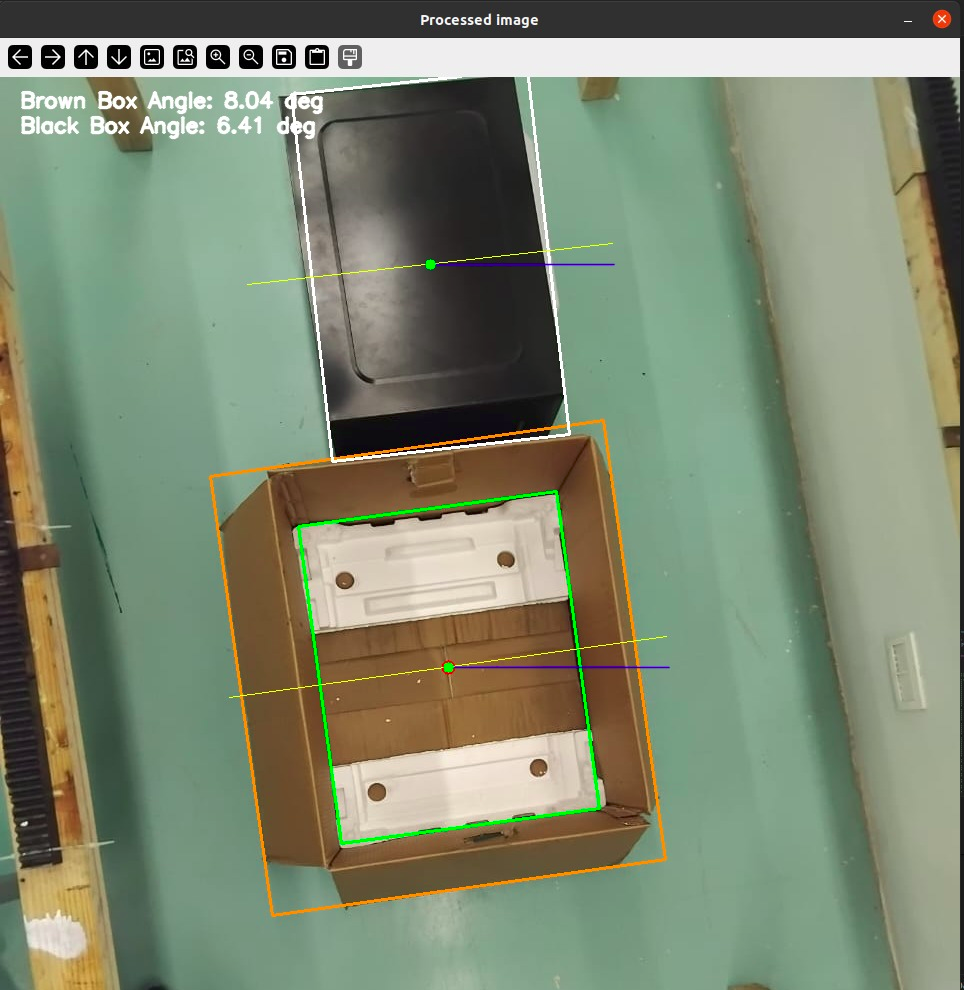
\includegraphics[width=0.6\linewidth]{figures/image_processing.png}
    \caption{Image processing performed on real data.}
    \label{fig:placeholder}
\end{figure}




% ============================================================
% Place this after the existing Capstone 1 content
% (after the image_processing.png figure and the paragraph
%  about real-world limitations)
% ============================================================
 
\section{Limitations of Classical Pipeline}
\label{sec:classical_limitations}
 
While the HSV-based segmentation pipeline demonstrated reliable performance in simulation, deployment on real hardware exposed several fundamental limitations. The flaps of the cardboard box and the recessed edges of the microwave introduced contour irregularities that degraded the accuracy of \texttt{cv2.minAreaRect}, particularly in position estimation. More critically, the pipeline exhibited the following structural shortcomings:
 
\begin{enumerate}
    \item \textbf{Color dependency:} HSV thresholding required manual tuning of per-object color ranges. Any change in object appearance, conveyor background, or lighting conditions necessitated recalibration, making the system fragile in uncontrolled environments.
    \item \textbf{Single-class limitation:} Each color range was hand-tuned for one object type. Extending the pipeline to new objects required defining additional masks, with no principled way to handle objects sharing similar color profiles.
    \item \textbf{No 3D pose:} The \texttt{minAreaRect} fit provided only a 2D center $(u, v)$ and an in-plane angle $\theta$. While sufficient for IBVS, this precluded metric-space control strategies that require the object's position and orientation in world coordinates.
    \item \textbf{No semantic keypoints:} The contour-based approach had no notion of specific object features (e.g., corners of the top face). Without known correspondences between image points and physical geometry, camera-to-object distance and full 6DoF pose could not be recovered.
\end{enumerate}
 
These limitations motivated a transition from classical image processing to a deep learning--based approach capable of jointly detecting objects, classifying them, and localizing semantically meaningful keypoints in a single forward pass.
 
\section{Deep Learning--Based Pose Estimation Pipeline}
\label{sec:dl_pipeline}
 
To address the shortcomings identified in Section~\ref{sec:classical_limitations}, the vision pipeline was redesigned around a keypoint-based pose estimation architecture. The revised pipeline, illustrated in Figure~\ref{fig:dl_pipeline_flow}, replaces HSV thresholding, morphological filtering, and contour extraction with a single neural network that simultaneously performs object detection (bounding box and class) and keypoint regression. The detected keypoints, corresponding to known physical corners of the target object, are then passed to a Perspective-n-Point (PnP) solver to recover the full 6DoF pose relative to the camera.
 
\begin{figure}[H]
    \centering
    % Replace with the exported pipeline flowchart
    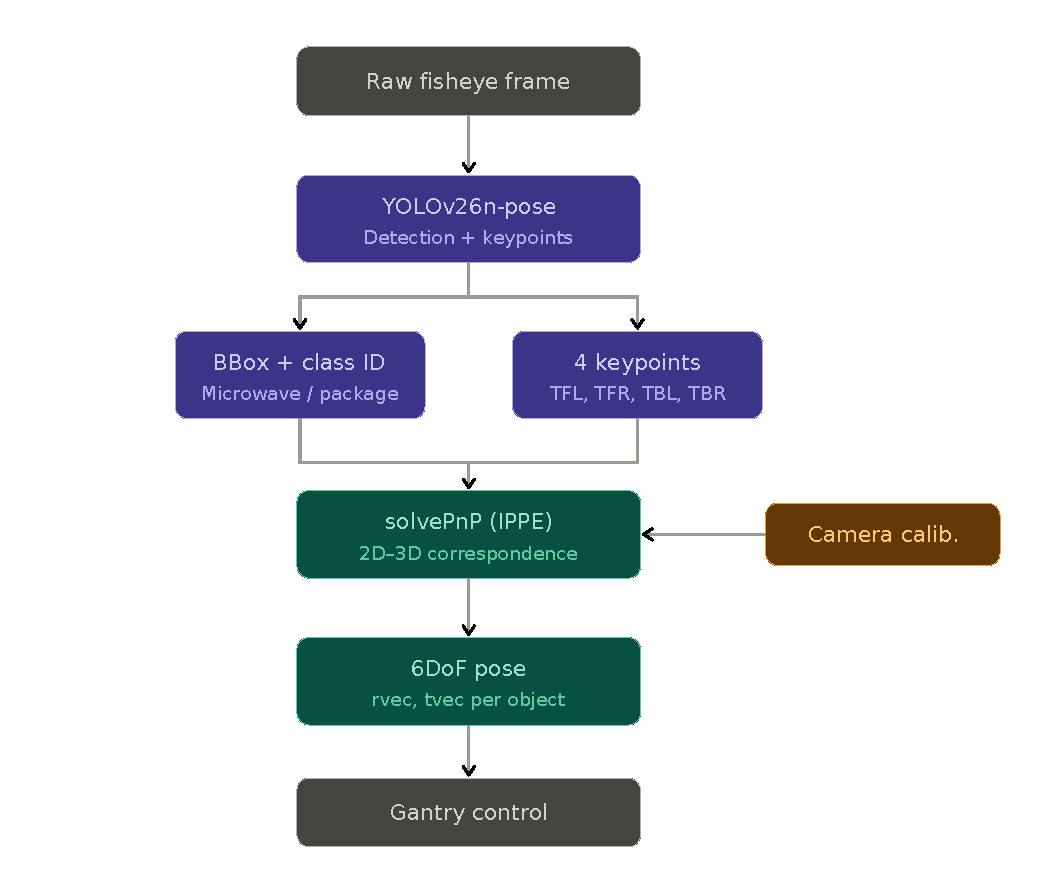
\includegraphics[width=\linewidth]{figures/dl_vision_pipeline_flowchart.pdf}
    \caption{Revised vision pipeline using YOLOv26n-pose for joint detection and keypoint regression, followed by PnP-based 6DoF pose estimation.}
    \label{fig:dl_pipeline_flow}
\end{figure}
 
This design choice offers three key advantages over the classical approach. First, the network learns appearance-invariant features from data, eliminating manual color tuning and providing robustness to lighting variation. Second, the architecture natively supports multiple object classes---in this case, microwaves and their packaging boxes---within a unified model. Third, by regressing semantically defined keypoints (the four top-face corners), the pipeline establishes the 2D--3D correspondences required for metric pose recovery via \texttt{cv2.solvePnP}, enabling position-based control strategies alongside or in place of IBVS.
 
The following sections detail the keypoint definition and dataset preparation (Section~\ref{sec:keypoint_def}), model architecture and training (Section~\ref{sec:model_training}), camera calibration (Section~\ref{sec:camera_calib}), and PnP-based pose recovery (Section~\ref{sec:pnp_pose}).
 


% ============================================================
% Continues from vision_transition.tex
% ============================================================

\section{Keypoint Definition}
\label{sec:keypoint_def}

The choice of keypoints is driven by two constraints: they must be consistently visible from the overhead wrist camera, and they must form a known planar geometry so that \texttt{cv2.solvePnP} can recover pose from a minimum of four 2D--3D correspondences. Because both the microwave and the cardboard package present a flat, roughly rectangular top face to the camera, the four corners of this face are selected as the keypoint set:

\begin{enumerate}
    \item \textbf{TFL} --- Top Front Left
    \item \textbf{TFR} --- Top Front Right
    \item \textbf{TBL} --- Top Back Left
    \item \textbf{TBR} --- Top Back Right
\end{enumerate}

\begin{figure}[H]
    \centering
    % Replace with annotated top-face keypoint diagram
    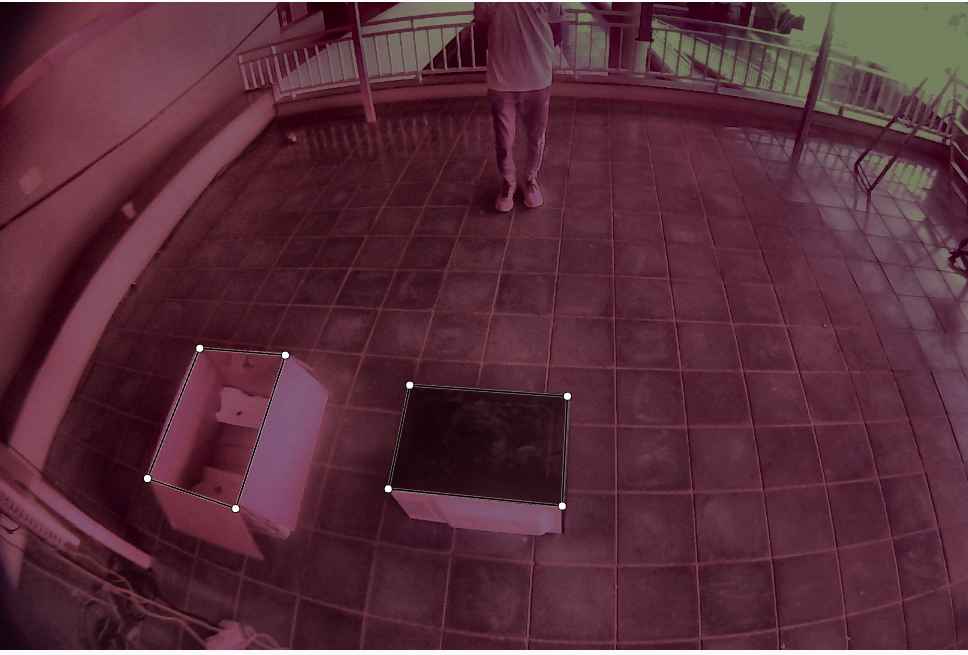
\includegraphics[width=0.55\linewidth]{figures/key-points.png}
    \caption{Keypoint convention for both object classes. TFL, TFR, TBL, and TBR denote the four corners of the top face as seen from the overhead camera.}
    \label{fig:keypoint_def}
\end{figure}

Since both classes share the same four-keypoint layout, a single model head can regress keypoints for all detections regardless of class. The keypoint ordering also defines a left--right mirror symmetry: under horizontal flip, TFL swaps with TFR and TBL swaps with TBR. This symmetry is encoded via the \texttt{flip\_idx: [1, 0, 3, 2]} field in the dataset configuration, enabling flip-based augmentation to preserve keypoint semantics.

Each keypoint is stored in the YOLO pose format as a triplet $(x, y, v)$, where $x$ and $y$ are normalized image coordinates and $v \in \{0, 1, 2\}$ is a visibility flag (0 = absent, 1 = occluded, 2 = visible). A label row thus contains 17 values: 5 for the bounding box (class, $c_x$, $c_y$, $w$, $h$) and $4 \times 3 = 12$ for the keypoints.

\section{Dataset Preparation}
\label{sec:dataset_prep}

The training dataset was assembled by merging three separate annotation efforts hosted on Roboflow, each created at a different stage of the project:

\begin{enumerate}
    \item \textbf{Old dataset} --- 8-keypoint COCO-format annotations for microwaves only (class = microwave). This dataset included all eight box corners; only the top four (indices 0--3) were retained during conversion.
    \item \textbf{Mid dataset} --- 4-keypoint YOLO-format annotations for microwaves only, already conforming to the top-face convention.
    \item \textbf{New dataset} --- 4-keypoint YOLO-format annotations with two classes: microwave (class 0) and package (class 1).
\end{enumerate}

Because the old dataset used COCO annotation format with eight keypoints per instance, a format-conversion script was written to: \textit{(i)} extract only the top-four keypoints by index, \textit{(ii)} convert bounding boxes from COCO absolute $(x, y, w, h)$ to YOLO normalized center format, and \textit{(iii)} hardcode the class ID to 0 (microwave). The mid and new datasets, already in YOLO pose format, were copied directly with class IDs preserved. All images and labels were merged into a single directory structure with unique filename prefixes (\texttt{old\_}, \texttt{mid\_}, \texttt{new\_}) to prevent collisions.

\begin{figure}[H]
    \centering
    % Replace with dataset merge pipeline diagram
    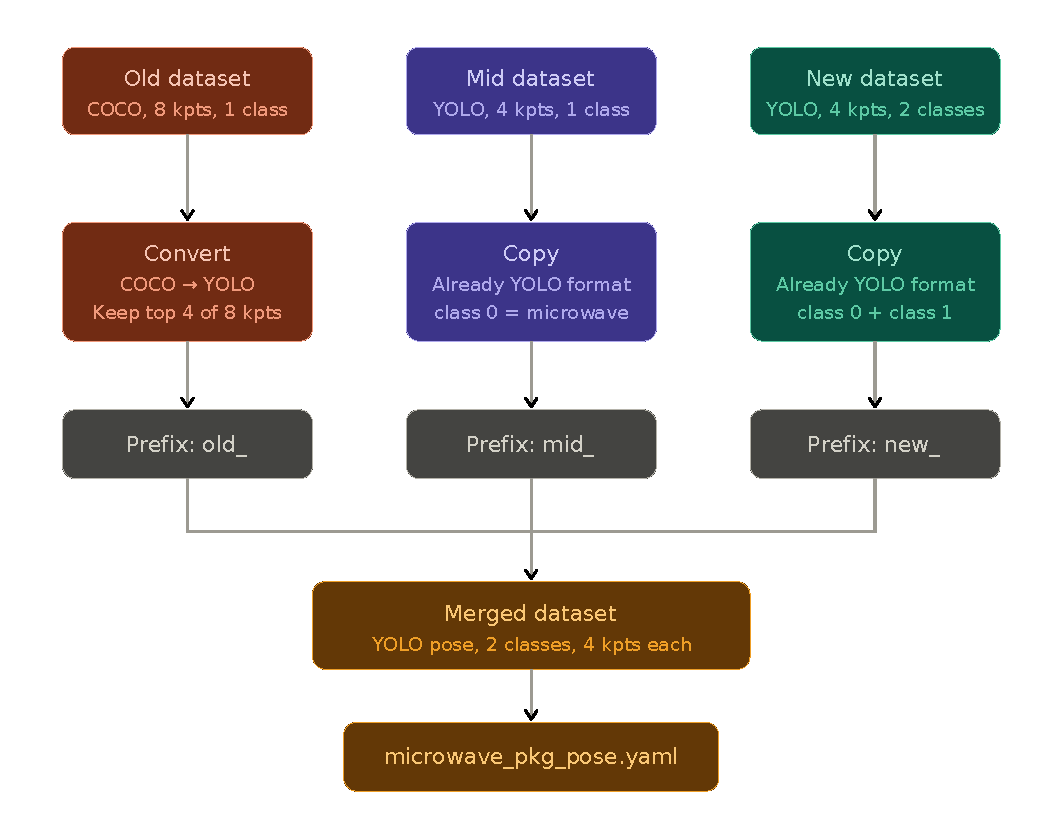
\includegraphics[width=0.85\linewidth]{figures/dataset_merge_pipeline.pdf}
    \caption{Dataset curation pipeline. Three annotation sources are converted to a unified YOLO pose format with 2 classes and 4 keypoints per instance.}
    \label{fig:dataset_merge}
\end{figure}

The final merged dataset configuration is specified in a YAML file consumed by the Ultralytics training API:

\begin{verbatim}
nc: 2
names:
  0: microwave
  1: package
kpt_shape: [4, 3]
flip_idx: [1, 0, 3, 2]
\end{verbatim}

% NOTE: Insert actual image counts from your training run here
% e.g., "The merged training set contains N_train images and the validation set contains N_val images."

\section{Model Architecture and Training}
\label{sec:model_training}

The detection and keypoint regression model is YOLOv26n-pose, a nano-variant of the YOLO architecture designed for real-time pose estimation. The model accepts a $640 \times 640$ input image and produces, for each detected object, a bounding box with class confidence and a set of $K$ keypoint coordinates with per-keypoint confidence scores. In this work, $K = 4$ corresponding to the top-face corners defined in Section~\ref{sec:keypoint_def}.

Training was initialized from the official \texttt{yolo26n-pose.pt} pretrained weights and fine-tuned on the merged dataset for 150 epochs with the following configuration:

\begin{table}[H]
    \centering
    \caption{YOLOv26n-pose training hyperparameters.}
    \label{tab:training_params}
    \begin{tabular}{ll}
        \hline
        \textbf{Parameter} & \textbf{Value} \\
        \hline
        Input size         & $640 \times 640$ \\
        Batch size         & 8 \\
        Epochs             & 150 \\
        Pretrained weights & \texttt{yolo26n-pose.pt} \\
        Flip LR / Flip UD  & 0.0 / 0.0 \\
        Mosaic             & 0.0 \\
        MixUp              & 0.0 \\
        Rotation / Perspective / Shear & 0.0 / 0.0 / 0.0 \\
        \hline
    \end{tabular}
\end{table}

A key design decision was the disabling of all geometric augmentations---horizontal/vertical flip, mosaic, mixup, rotation, perspective warp, and shear. While these augmentations are standard for object detection, they can corrupt keypoint semantics in pose estimation tasks. Mosaic and mixup composite multiple images, which can split an object's keypoints across tile boundaries or blend them with another instance. Similarly, large rotations and perspective warps alter the spatial relationship between keypoints in ways that the fixed \texttt{flip\_idx} mapping cannot account for. Since the gantry camera always views the conveyor from roughly the same overhead angle, the limited viewpoint variation in deployment further reduces the need for aggressive geometric augmentation.

% NOTE: Insert training results here once you have them
\subsection{Training Results}
Training curves for box loss, pose loss, and classification loss are shown in Figure~\ref{fig:training_curves}.
\begin{figure}[H]
    \centering
    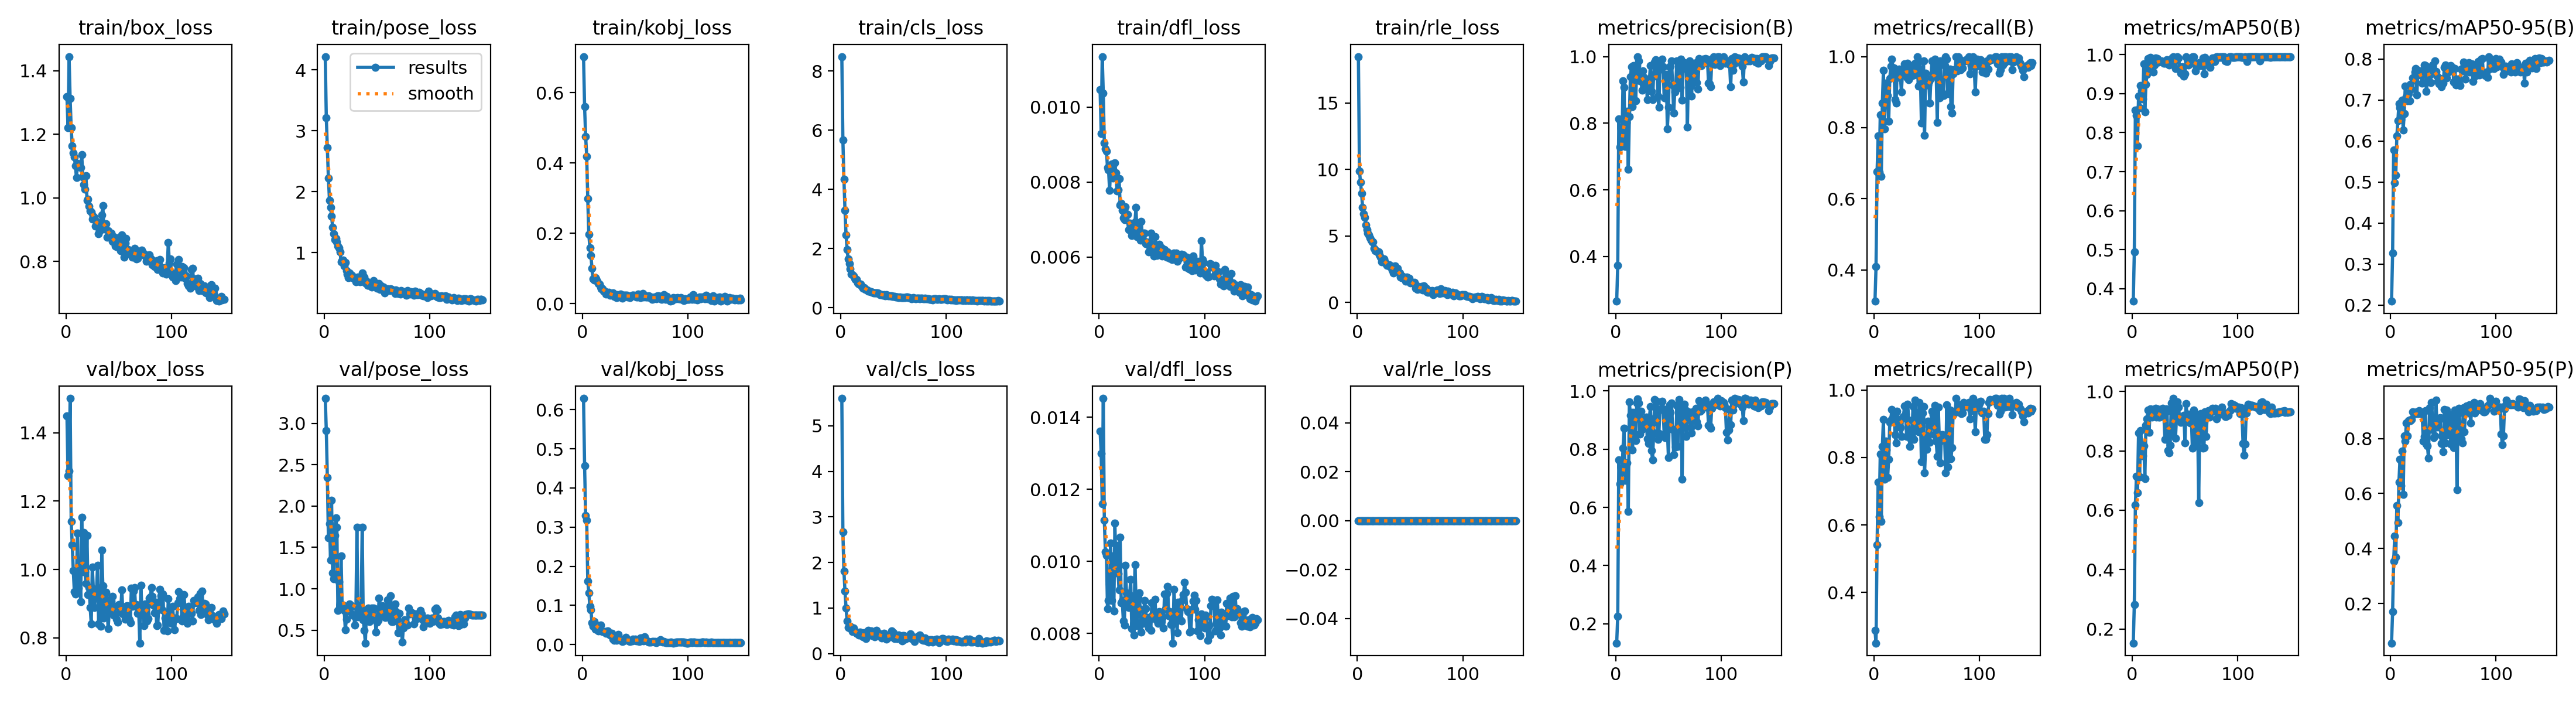
\includegraphics[width=\linewidth]{figures/vision-curves.png}
    \caption{Training and validation loss curves over 150 epochs.}
    \label{fig:training_curves}
\end{figure}
%
% Validation metrics:
% \begin{table}[H]
%     \centering
%     \caption{Validation performance of the trained YOLOv26n-pose model.}
%     \label{tab:val_metrics}
%     \begin{tabular}{ll}
%         \hline
%         \textbf{Metric} & \textbf{Value} \\
%         \hline
%         Box mAP@50       & X.XXXX \\
%         Box mAP@50--95   & X.XXXX \\
%         Pose mAP@50      & X.XXXX \\
%         Pose mAP@50--95  & X.XXXX \\
%         \hline
%     \end{tabular}
% \end{table}

\section{Camera Calibration}
\label{sec:camera_calib}

The wrist-mounted camera uses a fisheye lens to maximize the field of view over the conveyor. Fisheye lenses introduce significant radial distortion, particularly near the image periphery, which displaces pixel coordinates from their ideal pinhole-model positions. If uncorrected, this distortion degrades the accuracy of the PnP pose estimate.

Camera calibration was performed offline using an ArUco marker board. The calibration procedure yields two outputs:

\begin{itemize}
    \item The \textbf{intrinsic matrix} $\mathbf{K}$, containing the focal lengths $(f_x, f_y)$ and principal point $(c_x, c_y)$:
    \[
    \mathbf{K} = \begin{bmatrix} f_x & 0 & c_x \\ 0 & f_y & c_y \\ 0 & 0 & 1 \end{bmatrix}
    \]
    \item The \textbf{distortion coefficients} $\mathbf{d} = [k_1, k_2, p_1, p_2, k_3, \ldots]$, modelling radial and tangential lens distortion.
\end{itemize}

These parameters are stored in a NumPy archive (\texttt{camera\_params\_fisheye\_aruko.npz}) and loaded at inference time. Notably, the YOLO model runs on the raw distorted image; undistortion is deferred to the PnP stage, where the distortion coefficients are passed directly to \texttt{cv2.solvePnP}. This avoids the computational cost of undistorting the full frame at every inference step while still accounting for lens distortion during pose recovery.

\section{PnP-Based 6DoF Pose Recovery}
\label{sec:pnp_pose}

Given the four detected keypoints in pixel coordinates and the known physical dimensions of each object class, the Perspective-n-Point (PnP) algorithm recovers the 6DoF pose (rotation $\mathbf{R}$ and translation $\mathbf{t}$) of the object with respect to the camera frame.

\subsection{3D Object Model}

For each class, a planar 3D model is defined by placing the four top-face corners in a local object coordinate frame with the top surface at $Z = 0$:

\begin{table}[H]
    \centering
    \caption{3D object models for PnP. All keypoints lie on the $Z = 0$ plane.}
    \label{tab:object_models}
    \begin{tabular}{lcccc}
        \hline
        \textbf{Class} & \textbf{TFL} & \textbf{TFR} & \textbf{TBL} & \textbf{TBR} \\
        \hline
        Microwave & $(0, 0, 0)$ & $(0.44, 0, 0)$ & $(0, 0.61, 0)$ & $(0.44, 0.61, 0)$ \\
        Package   & $(0, 0, 0)$ & $(0.57, 0, 0)$ & $(0, 0.67, 0)$ & $(0.57, 0.67, 0)$ \\
        \hline
    \end{tabular}
\end{table}

\noindent Here, dimensions are in metres: the microwave top face measures $0.44 \times 0.61$\,m and the package measures $0.57 \times 0.67$\,m.

\subsection{Solver Configuration}

The PnP problem is solved using a two-stage fallback strategy. The primary solver is \texttt{SOLVEPNP\_IPPE} (Infinitesimal Plane-based Pose Estimation), which is specifically designed for coplanar point configurations and returns up to two candidate poses. If IPPE fails (e.g., due to near-degenerate keypoint configurations), the solver falls back to \texttt{SOLVEPNP\_ITERATIVE}, which uses Levenberg--Marquardt refinement from a DLT initial estimate.

The solver receives:
\begin{itemize}
    \item \textbf{Object points:} the 3D model coordinates from Table~\ref{tab:object_models}.
    \item \textbf{Image points:} the four keypoint pixel coordinates $(u_i, v_i)$ from the YOLO prediction, filtered by a per-keypoint confidence threshold of 0.30.
    \item \textbf{Camera matrix} $\mathbf{K}$ and \textbf{distortion coefficients} $\mathbf{d}$ from calibration.
\end{itemize}

\noindent The outputs are the rotation vector $\mathbf{r}$ (Rodrigues form) and translation vector $\mathbf{t}$, from which the full rotation matrix $\mathbf{R}$ can be recovered via the Rodrigues formula.

\subsection{Pose Interpretation}

From the recovered pose, two distance measures are computed:

\begin{enumerate}
    \item \textbf{Distance to object origin:} $d_{\text{origin}} = \|\mathbf{t}\|$, the Euclidean distance from the camera to the TFL corner.
    \item \textbf{Distance to object center:} The 3D center of the top face, $\mathbf{p}_{\text{obj}} = [W/2,\; D/2,\; 0]^T$, is transformed to camera coordinates via $\mathbf{p}_{\text{cam}} = \mathbf{R}\,\mathbf{p}_{\text{obj}} + \mathbf{t}$, and the distance is $d_{\text{center}} = \|\mathbf{p}_{\text{cam}}\|$.
\end{enumerate}

\subsection{Reprojection Error}

To assess the quality of each pose estimate, the 3D model points are reprojected back into the image using the recovered $\mathbf{r}$ and $\mathbf{t}$:

\[
\hat{\mathbf{p}}_i = \texttt{projectPoints}(\mathbf{P}_i, \mathbf{r}, \mathbf{t}, \mathbf{K}, \mathbf{d})
\]

The mean reprojection error is then:

\[
e_{\text{reproj}} = \frac{1}{4} \sum_{i=1}^{4} \| \hat{\mathbf{p}}_i - \mathbf{p}_i \|_2
\]

\noindent where $\mathbf{p}_i$ are the detected keypoints and $\hat{\mathbf{p}}_i$ are their reprojections. A low reprojection error (typically $< 5$\,px) indicates a geometrically consistent pose. This metric serves as an online quality gate: detections with high reprojection error can be rejected before being passed to the gantry controller.

\begin{figure}[H]
    \centering
    % Replace with solvePnP visualization (axes + keypoints + reprojected points)
    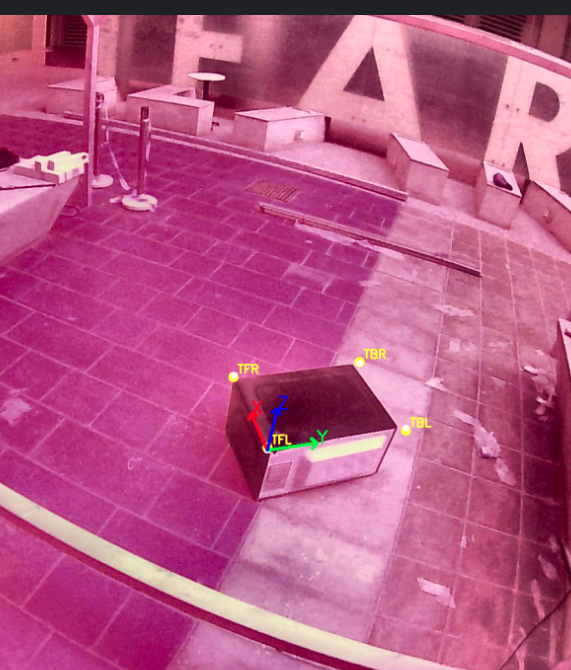
\includegraphics[width=0.7\linewidth]{figures/pnp-pose.png}
    \caption{PnP pose visualization on a validation image. Coloured dots are detected keypoints, white dots are reprojections, and RGB arrows indicate the recovered object-frame axes (X = red, Y = green, Z = blue).}
    \label{fig:pnp_vis}
\end{figure}
